\chapter{外文资料的书面翻译}

\title{一个基于互联网扫描的搜索引擎}

{\heiti 摘要:} 从揭开随机数量的发生器中的漏洞,到跟踪“心脏滴血”漏洞的进化中的影响,快速互联网扫描都为网络安全研究开启了新的领域。
然而,这项技术仍然需要进行更多的重要的工作:即使是简单的问题,比如,“什么模型的嵌入式设备更喜欢用CBC模式密码?”,需要开发一款扫描器软件,
人力地给设备分类并加标签,和网络管理员协商,并对辱骂的抱怨进行回复。在这篇论文里,我们将介绍一个基于一刻不停的互联网扫描采集的数据的,
公开的搜索引擎和数据处理设备,叫做Censys。Censys设计之初就是为了帮助研究人员解决安全相关问题,它支持协议头和很多的相关字段的全文搜索,
比如443.https.ciper。它能辨认具体的有漏洞的设备和网络,然后生成广泛使用的模式和趋势的数据报告。Censys可以在亚秒级时间内返回这些结果,
大大降低了理解构成互联网的主机的难度。我们将展示这个搜索引擎的结构,并通过实验来评估其性能。我们也将探索Censys的应用场景,
并展示这些在最近的研究中提出的问题是如何变得易于回答的。

\section{引言}
从最近骤增的基于快速互联网扫描的论文数量就可以看出,这项技术为经验驱动的安全研究开启了新的篇章。
然而即便如ZMap这样的扫描工具减少了执行大规模端口扫描工作的时间,通过互联网扫描来收集有意义的数据仍然是一项专业而且费力的工作。
回答类似“有多少HTTPS服务器更喜欢前向安全秘钥交换方式?”这样简单的问题可能需要数周的实现和调试,
减少了安全研究人员可以专注于其他更重要的问题上的时间。在这个具体的例子中,研究人员需要开发一款高性能的扫描软件,
通过HTTPS连接到正在监听443端口的主机,测试并修复一些主机因为没有完全遵从TLS协议的描述来实现而产生的问题,运行实际的扫描,
然后处理数GB的产生的结果数据。

在开始这个过程之前,安全研究人员必须和他们学院的法律和网络管理团队进行协商,来获得执行这个扫描的权限,和他们上游的网络提供商进行协调,
之后还要对辱骂的抱怨进行回应。很多学院(和独立研究者)缺乏网络设备或者行政权来执行扫描。因为这些原因,互联网扫描成为了一项鲜有研究者研究的领域,
严重地限制了这个强大的方法论的应用。

为了使互联网扫描民主化,和使研究人员可以有效地回答关于安全协议在实际中的使用和部署的问题,我们开发了Censys,
一个不仅维护了一个实时的互联网中IPv4地址空间中主机和服务的快照,而且为这些数据提供了搜索引擎和API的云服务。
和现有的主要专注于发现主机的扫描工具相比,Censys基于全部的协议握手快速地产生结果,
促进了一种社区驱动的描述爆炸性增长的网络中嵌入式主机和漏洞的方法,而且不需要或者需要很少任何用户的准备。

为了使该工具接近一个实时的互联网的鸟瞰图,Censys持续地在公共地址空间上扫描一系列重要端口和协议。
它检查这些数据的有效性并用可插拔的扫描框架并进行应用层的握手,而这个框架会仔细分析每次握手并产生关于每一个主机和协议的结构化数据。
产生的结果数据是经过后处理的,带有一个可扩展的标记框架,使得研究人员可以通过编程来定义额外的属性来分辨每个主机的设备的模型和标记和安全有关的属性。
我们透明地操作Censys并把数据直接暴露给研究社区。相应地,
我们希望外部研究人员为Censys贡献扫描软件(用来扫描更多的协议)和标记(用来分辨设备或属性)。以这种方法,Censys把扫描的机械操作自动化且中心化。

Censys把结果通过一个公开的搜索引擎,REST API,所有人都可以访问的Google BigQuery中的表和可以下载的数据集返回给研究人员。
搜索的接口使得研究人员可以进行全文搜索,也可以查询任意在扫描后和后处理后的结构化的字段和标记(比如443.https.cipher\_suite)。
它支持全文搜索,正则表达式搜索,和数据范围搜索,而且查询可以含有布尔逻辑。这些查询可以和谁都可以访问的目前的IPv4主机,
Alexa Top 1 Million中的网站和已知的X.509证书的快照进行竞争。在执行一次搜索后,用户可以互动地发现他们搜索的主机,站点和证书,
同时也会生成在研究中可以直接使用的数据报告。

举个简单的例子,Censys可以简单地通过443.https.heartbleed.vulnerable: true AND location.country\_code: 
US这条搜索词来分辨在美国的主机中有“心脏滴血”漏洞的主机。从这里,Censys可以输出一个完整的匹配的IP地址的列表,
并且能绘制出最常见的漏洞设备模型的分布图。这些查询都是在1秒内完成的。

为了便于更复杂的分析,我们发布原始应用程序握手和日常的时间点快照的结构化数据。 
这些数据可以通过SQL语句查询可公开访问的Google BigQuery表获得或以JSON格式下载。Censys的另一个提供数据的方式是一个公开的REST API,
允许研究人员导出原始数据查询结果,获取统计数据,查看特定主机和网络的历史状态。

我们将在第三部分中提供Censys的收集数据的架构,在第四部分中解释Censys如何向研究人员提供数据,并在第五部分描述我们是如何部署的。
接下来我们将在第六部分中展示Censys可以应用于轻松回答一系列有关最近的安全研究相关的问题的潜力,
其中包括衡量POODLE的影响和跟踪易受攻击的工业控制系统。

互联网扫描已经展示出应用于揭露安全问题和理解安全复杂的分布式系统的巨大的潜力。通过把扫描移到云端,Censys大大减少了调查这些问题需要的努力,使研究人员能够专注于提出更重要的问题而不是回答他们的机制。此外,Censys允许安全社区提高全球协议覆盖并提供一个易于处理的解决方案,以理解数量增加的互联网中的嵌入式设备。同时,它最大限度地减少研究小组的冗余扫描,并最小化将会到来的被网络运营商监控的网络拥堵。
Censys可以通过公开网站https://censys.io免费访问。


\section{互联网好公民}

与通过主动网络探索进行的任何研究一样,我们的工作提出了重要的伦理考虑。我们仔细考虑了实验测量并披露我们的结果的影响。在考量我们的影响时,
我们考虑了各种利益相关者,从我们当地的学院到互联网服务提供商和远程系统的所有者。虽然该社区尚未获得主动测量的健全的道德标准,
我们的考量遵循广泛的道德原则,如“门洛报告”中的内容,以及按照原来ZMap中工作方式中规定的道德规范工作。

我们和网络管理员,我们的部门、学院和机构的IT领导协商,同样也和我们的上游ISP协商,以确保我们的扫描不会对网络运营产生不利影响,
并且支持中心可以将外部查询传送给我们的团队。第二,我们表示了我们活动的良好意图。全部进行扫描的主机具有WHOIS记录并有反向DNS条目描述扫描的意图。
此外,每台进行扫描的主机在80端口上运行一个简单的网站来描述研究的目标,包括我们要收集的数据,以及如何与我们联系。
第三,我们欢迎用户的排除请求并在24小时内对请求做出回应。第四,全部扫描执行符合标准的握手; 我们不发送格式错误的数据包或握手。

公开扫描数据也会引起道德问题,因为它公开有关潜在脆弱系统的信息。为了尽量减少危害,我们故意选择收集和分发至少在原则上已经公开可见的数据。
我们的扫描器不尝试登录,部署任何攻击,或尝试访问非公共资源路径。此外,我们将退出扫描请求视为一项从搜索索引中删除的请求,
以允许远程管理员决定是否包括在Censys的公共接口中。之后,许多网络运营商在了解了我们测量工作的目标后表示支持,并邀请我们继续扫描他们。
最后,我们希望通过发布我们小心获得和妥善管理的扫描数据,我们可以减少需要由其他研究人员进行的互联网扫描,从而减轻目的地网络的整体负担。

相比之下,人们已经工人攻击者已经会通过僵尸网络和防弹托管服务提供商使用互联网扫描工具来查找存在漏洞的设备。因此,配置为公开公开数据的系统有一定风险。
Censys通过给研究人员提供可靠和符合伦理的数据的来源,使得合法的研究人员更好地研究和强化这些主机,来使这片场地平等。

\section{收集数据}

Censys的数据是通过横向扫描公共IPv4地址空间获得的,它由一系列扫描器池中的扫描器完成。首先,我们使用ZMap进行主机发现扫描,
用可插拔的应用程序扫描器与会响应的主机进行程序握手,并派生结构化字段(例如证书主体或TLS密码套件)握手。我们保存并发布原始握手,
但是也继续进一步处理,验证收集的扫描数据,提取有价值的字段和用额外的元数据标注握手,比如使用用户定义的注释的设备型号和软件版本。

结构化的带标注的数据然后流式传输到中央数据库ZDb,由其汇总水平扫描的结果,调整数据并更新综合记录,用来描述个人的IPv4主机,
Alexa Top 1 Million中的网站,以及维护所有发现的辅助收集X.509证书和公钥。ZDb流更改到下游服务并产生可发布的时间点的主机和网站的快照,
以及差量更新其证书和公钥的集合。

有几个观察导致了这个架构。首先,当横向扫描测量一项服务的一个方面时(例如,一个HTTPS服务器是否支持SSLv3),研究问题通常需要多次扫描。例如,
计算支持SSLv3的HTTPS服务器的百分比时,需要一个通用的TLS扫描和一个SSLv3扫描。同样,设备型号只能通过它的HTTP页面识别,
但是这个信息对于研究任何协议都是有用的。因此,尽管数据是根据协议收集的,但是应按主机分组。其次,我们的框架需要可扩展,并且便于社区的加入。
ZMap的成功大部分归功于用户的贡献探针模块,我们相信Censys也是如此。在嵌入式设备数量的爆炸式增长互联网,这对于标注主机和服务尤其正确。反之,
Censys需要透明地操作并将数据提供给社区。第三,扫描和标注的数量都会随着时间而增长;我们的架构应该线性变化来处理这个增加负载。

\begin{figure}[H]
  \centering
  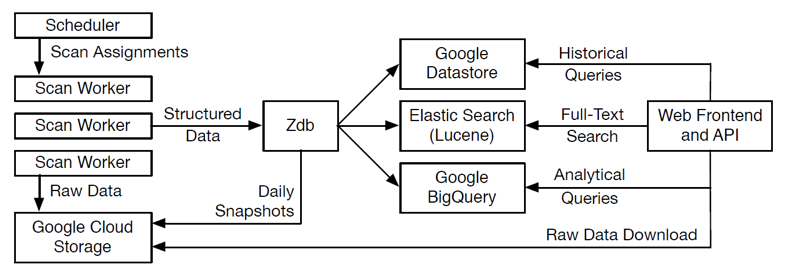
\includegraphics[scale=0.8]{censys-structure.png}
  \caption{{\heiti Censys系统体系结构} - Censys由IPv4地址空间的扫描应用程序驱动,它由一系列扫描器池中的扫描器完成。 
  这些扫描器完成扫描,提取有价值的字段,并标注记录额外的元数据,以便生成有关每个主机的结构化数据。 
  这些记录在一个中央数据库引擎ZDb中管理,它维护每个主机的当前状态。 ZDb将更新后的记录提交给Web前端,可供研究人员查询数据。}
  \label{fig:censys-structure}
\end{figure}

\subsection{互联网扫描}

在数据收集的第一步,我们使用ZMap来针对IPv4执行单包主机发现地址空间扫描。ZMap发现的主机作为可插拔应用程序扫描程序的种子,
用来执行后续的应用程序层握手并产生结构化的JSON数据,来描述主机是如何配置的的某个方面。通常情况下,
应用程序扫描程序只执行一次握手衡量服务配置的一个方面。例如,我们执行单独的横向扫描并使用不同的可插拔的扫描器来衡量HTTPS主机如何响应典型的TLS握手,
主机是否支持SSLv3,以及主机是否容易受到“心脏滴血”攻击。

{\heiti 可插拔的扫描器。}虽然我们可以使用ZMap来执行许多协议的主机发现,但是每个应用程序扫描器需要和协议相关的特定的代码,
而Censys的长期成功是因为它可以轻松添加新的协议。为了减少扫描新协议所需的工作量,Censys处理扫描的细节,并只需要最低限度的应用程序相关的扫描器。
具体而言,Censys需要一个自包含的Linux的可执行文件,它可以根据IP地址,通过stdin输入执行应用层握手,产生结构化的JSON输出,
在stdout上描述如何协议是如何配置的。Censys通过限制提供给扫描器的IP地址的速率控制网络带宽,用ZMap的内置分片工具分割扫描的多个扫描器,
并用ZMap的黑名单来保证应用程序扫描器不会扫描已经请求排除了的网络。

为了保护我们的基础设施,我们需要这个应用程序扫描程序不用root权限或内核操作修改就能工作。最后,我们鼓励研究人员输出JSON格式的扫描的元数据,
并用一个标准格式记录错误,使得Censys能够确认是否扫描已成功完成。我们希望通过要求最小的属性集,并允许语言的灵活性,
不仅可以减少我们团队添加额外的协议所需的工作量,还能鼓励外部社区开发新的扫描器。

{\heiti 扫描调度。}虽然立即测量协议的所有方面在技术上是非常简单的,但这经常涉及多次握手,这可能潜在地淹没主机(例如,
一个只允许同时一个或两个连接的嵌入式设备)。所以我们不这么做,而是选择独立执行扫描,依靠我们的数据处理流水线来聚合来自不同的数据扫描的数据,
以减少个别主机的负载。

在内部,扫描通过元组来引用(端口,协议,子协议,网络目的地),例如(443,https,heartbleed,ipv4\_shard1),
个人扫描的执行通过由扫描和时间戳引用。我们目前维护一个主扫描时间表; 我们计划自动规划扫描让它往后执行,以更好地分配网络负载。

\subsection{ZGrap:我们程序的扫描器}

我们正在发布一个快速和可扩展的应用程序扫描器,ZGrab,它符合之前描述的需求,也会促进新型扫描的快速发展。 目前,ZGrab支持HTTP,HTTP代理,
HTTPS,SMTP(S),IMAP(S),POP3(S),FTP,CWMP,SSH和Modbus的应用程序握手,以及StartTLS,Heartbleed,SSLv3和特定的密码套件检查。 
在带有Intel X520以太网适配器的双核Xeon E5-2640处理器上(6核2.5GHz),ZGrab可以在6小时20分钟内完成全部IPv4地址空间的HTTPS握手,
以及在3小时9分钟内完成一次banner-grab和所有可公开访问的SMTP的StartTLS连接主机,速度分别为1.86k和1.32k台主机每秒。

ZGrab是用Go实现的,我们选择Go是因为其原生的并发性,和其他低级语言相比安全性以及其原生的密码学库。该框架允许扫描器被定义为一个串行链的网络事件。
默认情况下,ZGrab对每台主机将只执行一个事件,连接,其行为只是打开一个TCP连接。最简单的事件可以是读取或写入数据,或更高级地,例如发起TLS握手。
例如,HTTPS扫描器被定义为一次连接事件和一次TLS握手事件。为了扩展ZGrab以支持扫描SMTP服务器之间的StartTLS支持,
我们添加了事件来读取SMTP的banner,写入SMTP EHLO命令,读取SMTP响应,发送StartTLS命令,读取响应,并执行TLS握手:总共62个LoC。
ZGrab框架处理并发连接,以及日志记录和生成描述连接的JSON文档。

原始的Censys部署中的所有协议都使用ZGrab,我们也鼓励其他研究人员考虑使用它作为开发其他应用程序扫描程序的起点。
我们正在发布和维护ZGrab作为一个独立的开源工具作为ZMap Project1的一部分。ZGrab可以独立于Censys使用,也可以结合ZMap使用:ZMap快速主机,
ZGrab产生关于每个主机的结构化数据。

\subsection{验证,提取和标注}

由可插入应用程序扫描器产生的原始JSON数据的由Censys收集,并在那里进行验证,转换成一个结构化的模式,并附加标注元数据(例如,设备制造商和型号),
然后才流入我们的中央数据库。

{\heiti 验证。}Censys以两种方式验证扫描数据。第一,我们扩展了ZMap来检测在主机发现阶段的网络响应的差异。如果扫描响应率在任何时候低于设定的阈值,
或者变化多于在扫描期间设置的数量,或者达到sendto失败的最大数量,或者如果libpcap跟不上导致丢失了设定数量的数据包,扫描自动终止并被重新安排。
其次,Censys在扫描完成时验证,并在ZMap或者应用程序扫描器的响应率低到一个静态边界时,或者在偏离之前两周的扫描的中位数超过了10\%时,拒绝这次扫描;
 被拒绝的扫描之后会手动检查。这些检查主要是为了检测瞬时网络故障,人为的配置错误和编码错误。

{\heiti 提取。}应用程序扫描仪输出与网络握手类似格式的,有关的原始数据应用程序握手的每个方面。例如,在TLS的情况下,
客户端和服务器的随机输出是客户端和服务器Hello消息的一部分。虽然这个数据是一些研究所需要的,但是很多这些字段都不是搜索主机或识别设备时有用的,
而且会导致我们的数据库中不必要的混乱。同样地,通常搜索的字段嵌套在网络的深处协议消息中,使它们很难被找到。
我们保存然后发布原始应用程序扫描器输出,但是也提取其中重要的值并转换握手数据为一种已经发布其格式的一致的结构化记录。这个过程中,
我们进一步以一种确定性的方式输出记录(即,如果没有记录更改了配置,则它们使用相同的加密哈希算法),
这使我们之后可以通过丢弃不包含更改的记录来减少负载。我们管这些表示服务配置的确定性记录叫做原子。

{\heiti 标注。}尽管应用程序扫描仪的输出可用于识别设备型号或版本,但这些细节不会被扫描器直接展示。相反,他们经常需要少量的逻辑
(例如,对HTTP服务器头或证书主体运行一个正则表达式)。为了方便添加这种类型的元数据,Censys允许研究人员定义标注 – 很小的函数 - 
可以给主机,网站和证书插入额外的元数据字段(例如,device\_module)或附加简单的标签(例如IPMI服务器的管理卡)。
注释被定义为对Censys从每次扫描生成的结构化数据只读的独立的Python函数。我们在图3中展示了一个用于标记Dell iDRAC远程管理卡的示例注释。

我们鼓励研究人员(和终端用户)贡献新类型的设备和漏洞注释。我们将在GitHub(http://github.com/zmap/ztag)
上托管我们的注释库和我们的转换和模式,作为一个独立的开源项目,ZTag。我们注意到,当ZTag与ZMap和ZGrab配合使用时,
研究人员可以独立重现Censys的数据处理流水线并产生相同的数据(图~\ref{fig:annotation})。

\begin{figure}[H]
  \centering
  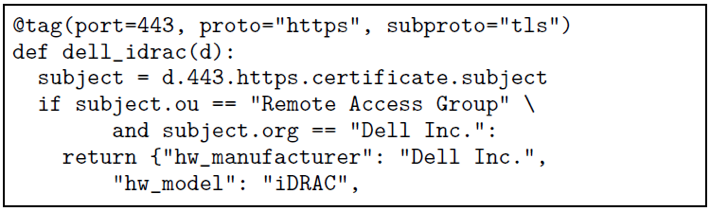
\includegraphics[scale=0.8]{annotation.png}
  \caption{{\heiti Dell iDRAC标注} - Censys支持社区维护标注 – 简单的Python函数 – 就能为记录附加额外的元数据和标签。
  在这里,我们展示了Dell iDRAC远程管理卡的标签。}
  \label{fig:annotation}
\end{figure}

\section*{翻译对应的原文索引}

\begin{translationbib}
\item Durumeric Z, Adrian D, Mirian A, et al. A search engine backed by internet-wide scanning
[C]//Proceedings of the 22nd ACM SIGSAC Conference on Computer and Communications
Security. [S.l.]: ACM, 2015: 542-553.
\end{translationbib}